\documentclass{beamer}

\usepackage{color}
\usepackage[T1]{fontenc}
\usepackage[utf8]{inputenc}
\usepackage{hyperref}
\usepackage{amsthm}
\usepackage{etoolbox}
\usepackage{mathtools}

\bibliographystyle{ieeetr}




\definecolor{WPI_red}{RGB}{172,43,55}
\setbeamertemplate{navigation symbols}{}
\setbeamertemplate{footline}[frame number]
\setbeamercolor{itemize item}{fg=WPI_red}
\setbeamercolor{itemize subitem}{fg=WPI_red}
\setbeamercolor{enumerate item}{fg=WPI_red}
\setbeamertemplate{caption}[numbered]
\setbeamercolor{caption name}{fg=WPI_red}
\setbeamertemplate{theorems}[numbered]
\renewcommand*{\thefootnote}{\fnsymbol{footnote}}
\setbeamercolor{block title}{use=structure,fg=white,bg=WPI_red}
\setbeamercolor{block body}{use=structure,fg=black,bg=WPI_red!5!white}
\renewcommand{\qedsymbol}{$\blacksquare$}
\undef{\lemma}
\newtheorem{lemma}{\translate{Lemma}}

\title{\textcolor{WPI_red} {Analysis of 5G Directional HetNets \\with Stochastic Geometry}}
% \subtitle{\color{black} Lecture 30}
\author{Travis Collins\\ Srikanth Pagadarai \\ Alexander Wyglinski}
\date{December 17, 2015}

\begin{document}

\frame{\maketitle}


\begin{frame}
\frametitle{\color{WPI_red} System Model}
\begin{itemize}

\item Desired signal is $S = r^{-\alpha}$.
\item Interference is modeled as \textit{shot noise}: 
\begin{equation*}
I = \sum_{x\in \Phi} h_x\;l(||x||)\; \zeta_{m, x}^2(\psi)
\end{equation*}
where, $h_x$ is an exponential random variable, $\Phi$ is a Poisson Point Process (PPP) and $\zeta_{m, x}(\psi)$ is the radiation pattern of the directional antenna - modeled as a Gaussian function~\cite{werner2015}. 

\item (Performance Metric) Probability of success: 
\begin{equation*}
p_s = P\left( \frac{S}{I} > \theta \right).
\end{equation*}

\end{itemize}

\end{frame}




\begin{frame}
\frametitle{\color{WPI_red} Probability of success for ALOHA}
\begin{itemize}

\item Interferers use omnidirectional antennas. Channel is Rayleigh and MAC scheme is ALOHA~\cite{haenggi2009}.
\begin{equation*}
p_s = exp\left(-p\lambda\pi r^2\theta^\delta\frac{\pi \delta}{sin(\pi\delta)}\right)
\end{equation*}
% \end{itemize}

\item Interferers use directional antennas. Channel is Rayleigh and MAC scheme is ALOHA.
\begin{equation*}
p_s = exp\left(-0.25p\lambda\sqrt{\pi} r^2\theta^\delta\frac{\pi \delta}{sin(\pi\delta)}\sqrt{\alpha\beta^2} erf\left(\frac{2\pi}{\sqrt{\alpha\beta^2}}\right)\right)
\end{equation*}



\end{itemize}

\end{frame}

\begin{frame}
\frametitle{\color{WPI_red} Probability of success for ALOHA}

\begin{figure}
    \centering
    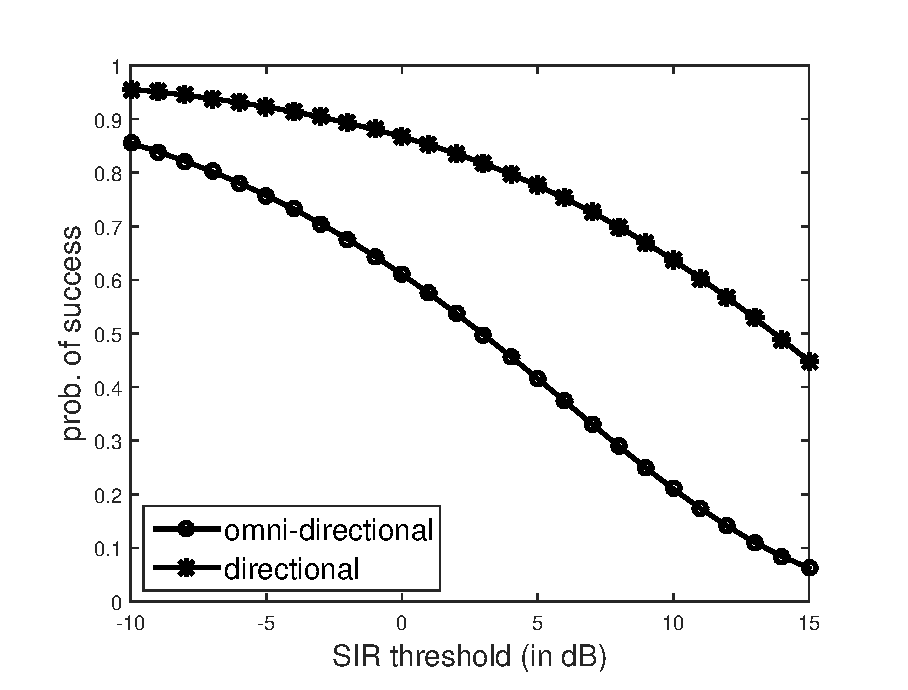
\includegraphics[resolution=2400, width=0.9\textwidth]{aloha.eps}
    \caption{Probability of success for ALOHA MAC when interferers use directional antennas ($\lambda=1/5$, $r=1$, $p=0.5$, $\beta=125.4^o$).}
\end{figure}



\end{frame}


\begin{frame}
\frametitle{\color{WPI_red} Probability of success for CSMA}
\begin{itemize}

\item Interferers use omnidirectional antennas. Channel is Rayleigh and MAC scheme is CSMA~\cite{haenggi2009}.
\begin{equation*}
p_s = exp\left(-p\lambda\pi \left(\eta+\frac{\rho^2r^2\theta^\delta}{r^2\theta^\delta+\rho^\alpha}\right)\right)
\end{equation*}

\item Interferers use directional antennas. Channel is Rayleigh and MAC scheme is CSMA.
\begin{equation*}
p_s = exp\left(-0.25p\lambda\sqrt{\pi}  \left(\eta+\frac{\rho^2r^2\theta^\delta}{r^2\theta^\delta+\rho^\alpha}\right)\sqrt{\alpha\beta^2} erf\left(\frac{2\pi}{\sqrt{\alpha\beta^2}}\right)\right)
\end{equation*}



\end{itemize}

\end{frame}



\begin{frame}
\frametitle{\color{WPI_red} Probability of success for CSMA}

\begin{figure}
    \centering
    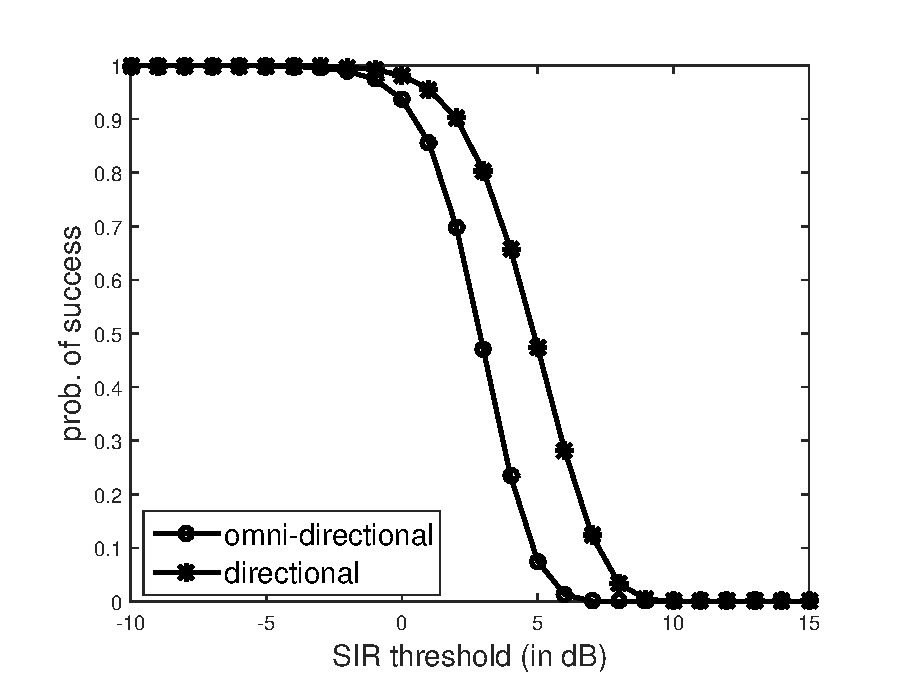
\includegraphics[resolution=2400, width=0.9\textwidth]{csma.eps}
    \caption{Probability of success for CSMA MAC when interferers use directional antennas ($\lambda=1/4$, $r=1$, $p=0.15$, $\beta=125.4^o$).}
\end{figure}



\end{frame}



\begin{frame}
\frametitle{\color{WPI_red} Future Work}
\begin{itemize}

\item A more detailed analytical evaluation of the relationship between antenna beamwidth and antenna mainbeam misalignment on the performance. 

\item Extend the probability of success performance metric by evaluating transmission capacity for directional networks using CSMA MAC scheme. 

\item The specific framework that will be used is the asymptotic SIR analysis work based on a PPP, in order to provide analytically tractable results for directional networks using CSMA. 
\end{itemize}

\end{frame}

\begin{frame}{Bibliography}
\bibliography{meeting_bib}
\end{frame}


\end{document}